\documentclass[11pt]{article}
\usepackage{amssymb,amsmath,amsthm}
\usepackage{setspace}
%\setlength{\parindent}{0.0in}

\theoremstyle{plain}
\newtheorem{theorem}{Theorem}[section]
\newtheorem{proposition}[theorem]{Proposition}
\newtheorem{lemma}[theorem]{Lemma}
\newtheorem{corollary}[theorem]{Corollary}
\newtheorem{conjecture}[theorem]{Conjecture}

\theoremstyle{definition}
\newtheorem{definition}[theorem]{Definition}
\newtheorem{exer}[theorem]{Exercise}
\newtheorem{remark}[theorem]{Remark}
\newtheorem{example}[theorem]{Example}

\newcommand*\conj[1]{\bar{#1}}
\newcommand{\overbar}[1]{\mkern 1.5mu\overline{\mkern-1.5mu#1\mkern-1.5mu}\mkern 1.5mu}



\title{\bf{Title}}
\begin{document}
\author {A Senior Comprehensive Project \\
by\\
name \\
Allegheny College\\
Meadville, PA}

\maketitle
\thispagestyle{empty}
\begin{center}
Submitted to the Department of Mathematics in partial fulfillment of the requirements for the degree of Bachelor of Science.
\end{center}

\vspace{0.5 in}
\begin{center}
Project Advisor:  Dr. Rachel J. Weir \\
Second Reader: [Enter name here.]
\end{center}

\vspace{0.5 in}
\begin{center}
I hereby recognize and pledge to fulfill my responsibilities, as defined in the Honor Code, and to maintain the integrity of both myself and the College community as a whole.
\end{center}

\vspace{0.25 in}
\begin{center}
Pledge:

\vspace{0.5 in}
-----------------------------------------------------------------

\vspace{0.00 in}
name
\end{center}

\newpage
\thispagestyle{empty}
\begin{center}
Acknowledgements
\end{center}
\doublespacing
%\hspace{0.5 in}  
I want to thank everybody for everything.  Keep typing to see what happens with a new paragraph.

Start a new paragraph thanking people.

\newpage

\thispagestyle{empty}

\begin{abstract}
This comp is about everything!
\end{abstract}
\newpage
\thispagestyle{empty}
\tableofcontents

\newpage
\doublespacing
\setcounter{page}{1}
\section{Introduction}
%\hspace{0.5 in}  

This purpose of this comp is to show that I've learned something really wonderful.

As a bonus, when I'm done and have passed the oral exam, I will finally graduate!


\newpage
\section{Preliminaries}
The purpose of this section of the paper is to review and expand on some of the more basic mathematical topics which are important in \authorsetals paper.  We review topics in metric spaces, complex analysis, and a few things from linear algebra.  These topics are the basic building blocks we need to understand some of the more advanced concepts in the paper.

\subsection{Metric Spaces}
Here we overview some elementary topological concepts about metric spaces.  We specifically talk about metric and vector spaces, norms, and the completion of metric spaces.  Note that many definitions, theorems, etc. come from Gerald Edgar's \textit{Measure, Topology, and Fractal Geometry}\cite{Edgar} and Kaplansky's \textit{Set Theory and Metric Spaces}\cite{Kaplansky}.

\begin{defn}
A \textbf{metric space} is a set $S$ together with a function $d:S \times S \rightarrow [0, \infty)$ satisfying the following:
\begin{align*}
\textrm{(1)}\; d(x,y) &= 0 \Leftrightarrow x = y\\
\textrm{(2)}\; d(x,y) &\geq 0 \textrm{ for all } x,y \in X\\
\textrm{(3)}\; d(x,y) &= d(y,x)\\
\textrm{(4)}\; d(x,z) &\leq d(x,y) + d(y,z) \textrm{ (Triangle inequality)}
\end{align*}
The nonnegative real number $d(x,y)$ is called the \textit{distance} between $x$ and $y$, while the function $d$ itself is known as the \textit{metric} of the set $S$.  A metric space is written as $(S, d)$, but oftentimes the metric is implied and the space is simply referred to as $S$.  Note that the last property, the triangle inequality, is a very important property as it is used very often in proofs.
\end{defn}

\begin{example}
The set of real numbers $\mathbb{R}$, with $d: \mathbb{R} \times \mathbb{R} \rightarrow \mathbb{R}$ defined by
\[d(x,y) = |x - y| \]
is a metric space.  This is the usual metric used with $\mathbb{R}$.
\end{example}

The complex plane $\mathbb{C}$ has a similar usual metric:

\begin{example}
The complex numbers $\mathbb{C}$ with $d: \mathbb{C} \times \mathbb{C} \rightarrow \mathbb{R}$ defined by
\[d(z,w) = |z - w| \]
where $|z|$ is the modulus of $z$ is a metric space.
\end{example}

Generally, algebraic operations are not defined on a metric space, just a distance function.  Meanwhile, a vector space (which is not necessarily a metric space) provides the operations of vector addition and scalar multiplication, but without a notion of distance.  We can combine a vector space with a \textit{norm}, though, to create a normed vector space --- note that all normed vector spaces are also metric spaces.

\begin{defn}
A \textbf{norm} on a vector space $V$ is a function $||x||: V \rightarrow [0, \infty) \subset \mathbb{R}$ which satisfies the following:
\begin{align*}
&\textrm{(1)}\; ||x|| \geq 0 \textrm{ and } ||x|| = 0 \textrm{ if and only if } x=0;\\
&\textrm{(2)}\; ||kx|| = |k|\,||x|| \textrm{ (scaling property)};\\
&\textrm{(3)}\; ||x + y|| \leq ||x|| + ||y||.
\end{align*}

A vector space $V$ together with a norm $||\cdot||$ is called a \textbf{normed vector space}, and is denoted $(V, ||\cdot||)$.
\end{defn}

The properties of a norm on a vector space are rather intuitive.  Property (1) says that a vector has nonnegative length, and the length of $x$ is 0 if and only if $x$ is the 0-vector; property (2) states multiplying a vector by a scalar $k$ multiplies its length by $k$; finally property (3) is the triangle inequality, which is analogous to property (4) of definition 3.1.

While a norm is defined rather similarly to a metric, the two are not the same.  However, we often define a metric on a normed metric space using the norm.

\begin{prop}
If $(X, ||\cdot||)$ is a normed vector space $X$, then $d: X \times X \rightarrow \mathbb{R}$, defined by $d(x,y) = ||x - y||$, is a metric on $X$.
\end{prop}

The necessary properties for $d$ to be a metric follow immediately from properties (1) and (3) of a norm.  If $X$ is a normed vector space, we always use the metric associated with its norm, unless specifically stated otherwise.

A metric defined on a norm has all the properties of a metric discussed earlier, as well as two more --- for all $x, y, z \in X$ and $k \in \mathbb{R}$
\[d(x+z, y+z) = d(x+y), \qquad d(kx, ky) = |k|d(x,y).\]

These properties are called \textit{translation invariance} and \textit{homogeneity}, respectively.  These properties are not included in a simple metric space because they do not even make sense in that framework --- recall that in a space which is only a metric space, we can not add points together or multiply them by scalars.

While there are a variety of norms which can be used on a vector space, the \textit{Euclidean norm} is the most common for $\mathbb{R}^n$ and is perhaps the most intuitive.

\begin{example}
On $\mathbb{R}^n$, the length of a vector $x = (x_1, x_2, ..., x_n)$ is given by
\[||x|| := \sqrt{x_1^2+x_2^2+\cdots+x_n^2}.\]
This gives the distance from the origin to the point $x$ and is known as the \textit{Euclidean norm}.  This should be familiar as it is the "straight-line" distance between points in space and is a result of the Pythagorean theorem.
\end{example}

\begin{example}
On $\mathbb{C}^n$, the most common norm is given by
\[||z|| := \sqrt{|z_1|^2 + |z_2|^2 + \cdots + |z_n|^2} = \sqrt{z_1\conj{z}_1 + z_2\conj{z}_2 + \cdots + z_n\conj{z}_n}\]
\end{example}

Note that while a metric is often derived from a norm, the existence of a metric does not imply a norm --- a metric does not even necessarily need to make geometric sense.  Take for example what is known as the \textit{discrete metric}:

\begin{example}
On any set $X$, the discrete metric is defined as
\[d(x,y)= 
\begin{cases} 
	0 & x=y, \\
	1 & x \neq y.\\
\end{cases}
\]
\end{example}

The discrete metric above does not satisfy the homogeneity property we briefly discussed earlier, so we know this metric was not induced by a norm.  However, if the metric of a metric space $V$ satisfies both the homogeneity and translation invariance properties, the metric $d$ can be used to define a norm $||\cdot||$ by
\[||x|| = d(x,0)\]
for all $x \in V$.

We now move on to a final important aspect of metric spaces: completeness of metric spaces and the completion of metric spaces.  First, we review a couple concepts about sequences.

\begin{defn}
A \textbf{sequence} is a function whose domain is a set of the form $\{n \in \mathbb{Z} : n \geq m\}$ for some $m \in \mathbb{Z}$.  A sequence is denoted $(s_n)_{n=m}^\infty$ or just $(s_n)$.
\end{defn}

\begin{example}
The following are a couple examples of sequences:
\begin{itemize}
\item Let $s_n = \frac{1}{n^2}, n\geq 1$.  Then, $(s_n) = (1, \frac{1}{4}, \frac{1}{9}, , \frac{1}{16}, \dots)$.
\item Let $s_n = \frac{1}{2}(1 + (-1)^n), n \geq 1$.  Then, $(s_n) = (0,1,0,1,\dots)$.
\end{itemize}
\end{example}

\begin{defn}
A sequence $(s_n)$ \textbf{converges} to a point $s$ provided that, for every $\epsilon \geq 0$, there exists an $N$ such that
\[n > N \Rightarrow d(x_n, s) < \epsilon.\]
This point $s$ is called the \textit{limit} of the sequence.  We denote the limit as $\lim(s_n) = s$.
\end{defn}

Essentially, a sequence converges to a point $s$ if, after some point in the sequence, all the terms are arbitrarily close to the limit.

\begin{defn}
Let $(X,d)$ be a metric space.  A sequence $(x_n)_{n=1}^\infty$ in $X$ is a \textbf{Cauchy sequence} if, for every $\epsilon > 0$, there exists an $N$ such that
\[n,m \geq N \Rightarrow d(x_n, x_m) < \epsilon.\]
\end{defn}

The definition of a Cauchy sequence is very close to that of a convergent sequence --- a Cauchy sequence, though, says that beyond some point in the sequence, all the terms are arbitrarily close to one another.  The two are closely related, and in fact imply one another.

\begin{theorem}
A sequence converges if and only if it is Cauchy.
\end{theorem}

The idea here is that, if a sequence converges, all the terms are eventually close to the same limit.  Since the terms are all close to the same limit, they are also very close to one another.  The same reasoning can be used to show that all Cauchy sequences converge.  We provide here a short proof for the forward direction.  Note the use of the triangle inequality property of metric spaces to prove this result.

\begin{proof}
We show that all convergent sequences are Cauchy.\\
Let $s = \lim(S_n)$.  Let $\epsilon > 0$.  Since $\lim(s_n) = s$, there exists $N$ for which $n > N \Rightarrow d(s_n, s) < \frac{\epsilon}{2}$.  So suppose $m,n > N$.  Then \begin{align*}
d(s_n, s_m) &\leq d(s_n, s) + d(s, s_m)\\
&< \frac{\epsilon}{2} + \frac{\epsilon}{2}\\
&= \epsilon.
\end{align*}
Thus by definition $(s_n)$ is Cauchy.
\end{proof}

\begin{defn}
A metric space $(X, d)$ is called \textbf{complete} if every Cauchy sequence in $X$ converges to some point in $X$.
\end{defn}

\begin{example}
Consider the sets $\mathbb{Q}, \mathbb{R}, \mathbb{C}$:
\begin{itemize}
\item The metric space $(\mathbb{Q}, d)$ where $d(x,y) = |x - y|$ (the usual metric for $\mathbb{Q}$) is not complete.  This is because there are sequences in $\mathbb{Q}$ which converge to irrational limits.  For example, 
\[(s_n) = \biggl ( 1 + \frac{1}{n} \biggr )^n\]
converges to $e$ which is not in $\mathbb{Q}$.

\item The metric spaces $(\mathbb{R}, d_1)$ and $(\mathbb{C}, d_2)$ with their usual metrics $d_1$ and $d_2$ respectively, are both complete.
\end{itemize}
\end{example}

Note that complete normed vector spaces are a special subset of metric spaces, known as \textit{Banach Spaces}.  Banach Spaces have several special properties and are an important concept in Jim{\`e}nez-Munguia \etals paper.  We discuss Banach Spaces in-depth in a later section of this paper.
\newpage
\subsection{The Complex Plane}
\authorsetals work is done entirely in the complex plane.  In this section we review the complex numbers and some topological concepts of the complex plane.  Most definitions and theorems are borrowed from \textit{Fundamentals of Complex Analysis} by Saff and Snider \cite{Saff}.

If we picture the real numbers $\mathbb{R}$ as a one-dimensional number line, the set of complex numbers $\mathbb{C}$ can be thought of as a plane with $\mathbb{R}$ as its x-axis and the set of imaginary numbers as its y-axis.  Then, an element of $\mathbb{C}$  consists of both a real part and an imaginary part.

\begin{defn}
A \textbf{complex number} is an expression of the form $a + bi$ where $a, b \in \mathbb{R}$, and $i$ is defined as the imaginary number $\sqrt{-1}$.  Two complex numbers $a+bi$ and $c+di$ are said to be equal if and only if $a=c$ and $b=d$.
\end{defn}

So, for a complex number $z = a + bi$, $a$ is said to be the real part (denoted Re $z$) and $b$ is the imaginary part (denoted Im $z$).  With this notation we can write $z = \textrm{Re }z + i \textrm{ Im }z$.  Note that if $b=0$, then $z$ is a real number, while if $a=0$, then $z$ is a pure imaginary number.

Recall that the complex plane $\mathbb{C}$ can be combined with a distance function $d$:
\[d(z,w) = |z-w|\] where $z,w \in \mathbb{C}$ and $|z|$ is the modulus of $z$ defined as below.  Furthermore, this metric is induced by the usual norm of $\mathbb{C}$: $||z|| = \sqrt{x^2 + y^2}$ where $z = x+iy$ for $x,y \in \mathbb{R}$.  From this point on, this metric will be implied when we refer to $\mathbb{C}$ .

\begin{defn}
The \textbf{modulus} or (\textbf{absolute value}) of a number $z = a + bi$ is denoted $|z|$ and is given by
\[|z| := \sqrt{a^2 + b^2}\]
\end{defn}

Note that $|z|$ is always a nonnegative real number, and the only complex number whose modulus is zero is the number 0 itself.

The reflection of a point $z=a+bi$ across the real axis is the point $a-bi$.  The relationship between a number and its reflection plays a large role in complex analysis.

\begin{defn}
The \textbf{complex conjugate} of a number $z=a+bi$ is denoted $\conj{z}$ and is given by
\[\conj{z} := a-bi.\]
\end{defn}

The conjugate is important due to the numerous properties regarding the possible interactions between a complex number and its conjugate.

\begin{example}
First, it is clear that $z=\conj{z}$ if and only if $z$ is a real number.  Furthermore, the conjugate of the sum/difference of two complex numbers is equal to the sum/difference of their conjugates.  That is,
\[\overbar{z_1 + z_2} = \overbar{z_1} + \overbar{z_2}, \;\; \overbar{z_1 - z_2} = \overbar{z_1} - \overbar{z_2}.\]
Beyond these two properties are a number of other ones as well:
\begin{itemize}
\item $\overbar{(z_1z_2)} = \overbar{z_1}\,\overbar{z_2}$\\
Indeed, if $z_1 = a+bi$ and $z_2 = c+di$, then
\vspace{-1em}
\begin{align*}
\overbar{z_1z_2} &= \overbar{ac - bd + (ad + bc)i}\\
&= ac - bd - (ad + bc)i\\
&= ac - bd - adi - bci\\
&= (a - bi)(c-di)\\
&= \overbar{z_1}\,\overbar{z_2}.
\end{align*}
\item In addition, the following can be seen:
\[\overbar{\biggl(\frac{z_1}{z_2}\biggr)} = \frac{\overbar{z_1}}{\overbar{z_2}}, \; (z_2 \neq 0);\]
\[\textrm{Re } z = \frac{z+\overbar{z}}{2};\]
\[\textrm{Im } z = \frac{z-\overbar{z}}{2i}.\]
The last two properties demonstrate that the sum of a number and its conjugate is real, and the difference is imaginary, respectively.
\item The conjugate of a conjugate is, of course, the original number:
\[\overbar{(\overbar{z})} = z.\]
The final two properties are specifically used in \authorsetals paper:
\[|z| = |\overbar{z}|, \;\; z\overbar{z} = |z|^2.\]
The first of these is easy to see geometrically (Figure 1).

\begin{figure}[h]
\centering
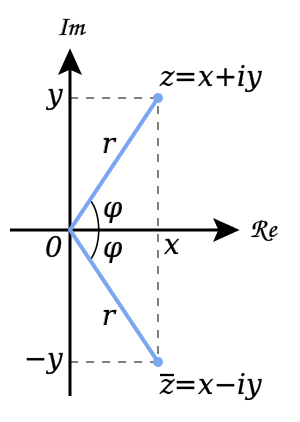
\includegraphics[scale=0.4]{images/complexmod.png}
\caption{Complex number and its modulus\cite{modulusimage}}
\end{figure}

The second can be proved easily:
\[z\overbar{z} = (a+bi)(a-bi) = a^2 + b^2 = |z|^2.\]
\end{itemize}
\end{example}

For functions of a real variable, we typically work with functions defined on an \textit{interval}, but this concept does not work for $\mathbb{C}$.  We must instead define some topological concepts for $\mathbb{C}$.

\begin{defn}
The \textbf{open disk} or \textbf{circular neighborhood} of a point $z_0$ is the set of all points $z$ which satisfy the inequality
\[|z-z_0| < p,\]
where $p$ is a positive real number.  This set consists of every point that lies inside the circle of radius $p$ around the center $z_0$.
\end{defn}

\begin{example}
The solution sets of the inequalities
\[|z-2| < 5, \;\;\; |z+i| < \frac{1}{2}, \;\;\; |z| < 8\]
are open disks centered at $2$, $-i$, and $0$ respectively.
\end{example}

A frequently used neighborhood is the \textit{open unit disk}:

\begin{defn}
The \textbf{open unit disk}, denoted $\mathbb{D}$ is as follows:
\[\mathbb{D} := \{z : |z| < 1\}.\]
\end{defn}

We will now define several closely related topological terms regarding sets.  We start with two terms in a single definition --- a two-for-one special, if you will.
\begin{defn}
For any set $S$, a point $z_0$ is called an \textbf{interior point} of $S$ if there is some open disk centered at $z_0$ which is completely contained in $S$.  If every point in $S$ is an interior point of $S$, we describe $S$ as an \textbf{open set}. 
\end{defn}

\begin{defn}
An open set $S$ is said to be \textbf{connected} if every pair of points can be joined by a curve which does not leave the set.  Alternatively, $S$ is connected if for all $p,q \in S$ there exists a finite collection of line segments contained in $S$ which join $p$ and $q$
\end{defn}

Essentially, a set is connected if it is a "single piece", geometrically speaking.  A \textit{convex set} is slightly more than this:

\begin{defn}
A set $S \in \mathbb{C}$ is said to be \textbf{convex} if
\[tp+(1-t)q \in S\]
for all $p,q \in S$ and for all $0 \leq t \leq 1$.  More simply, a set $S$ is convex if, for every pair of points in $S$, the line connecting the two points is contained within $S$.
\end{defn}

Note that, intuitively, all convex sets are connected, but a connected set is not necessarily convex.  Figure 2 shows this with geometric representations of sets --- (a) is both convex and connected, (b) and (c) are connected but not convex, and (d) is neither connected nor convex.

\begin{figure}[h]
\centering
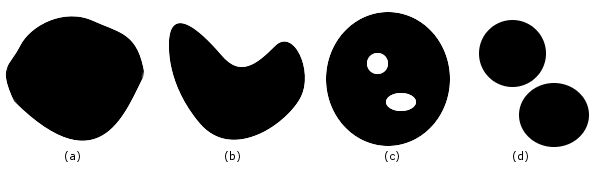
\includegraphics[scale=0.5]{images/convexvconnected.png}
\caption{Convex vs. Connected Sets}
\end{figure}

\begin{defn}
A point $z_0$ is said to be a \textbf{boundary point} of a set $S$ if every neighborhood of $z_0$ contains at least one point of $S$ and at least one point not in $S$.  Simply put, $z_0$ is a boundary point if it exists on the edge of the set.  The set of all boundary points is called the \textbf{boundary} of $S$, and we will denote this $\partial(S)$.
\end{defn}

\begin{defn}
A set $S$ is said to be \textbf{closed} if it contains all of its boundary points.  Equivalently, $S$ is closed if its complement $\mathbb{C} \ S$ is open.
\end{defn}

\begin{example}
Let $\overbar{\mathbb{D}} = \{z : |z| \leq 1\}$.  This is a closed set, as it contains its boundary $\partial(\mathbb{D}) = \{z : |z| = 1\}$.  $\overbar{\mathbb{D}}$ is known as the \textit{closure of $\mathbb{D}$} or the \textit{closed unit disk}.
\end{example}

The final topological concepts we need for $\mathbb{C}$ are those of \textit{boundedness} and \textit{compactness}.

\begin{defn}
A set of points $S$ is said to be \textbf{bounded} if there exists some $r \in \mathbb{R}^+$ such that $|z| < r$ for every $z$ in $S$.  Equivalently, $S$ is bounded if it is contained in any neighborhood of the origin.  $S$ is \textbf{unbounded} if it is not bounded.
\end{defn}

\begin{defn}
A set that is both closed and bounded is said to be \textbf{compact}.
\end{defn}

We have sufficiently described the complex space $\mathbb{C}$ as an extension of the real numbers.  Furthermore, we have outlined a number of topological concepts for $\mathbb{C}$.  Later on, in the section on Conformal Mappings, we explore concepts from complex analysis much deeper --- specifically, we will describe analytic functions of the complex variable from a geometric standpoint.
\newpage
\subsection{Eigenvalues}
asd
\newpage
\subsection{Linear Transformations}
linear trans

\newpage
\section{Chaos}
The following is a well known criterion for chaos, known as the Eigenvalue Criterion.  [2,3] provide proofs for the Criterion, and [9,10,12,14,15] provide examples using the Criterion.

\begin{theorem}
Let $T:X \rightarrow X$ be an operator on a separable complex Banach space $X$.  Consider the subspaces
\[X_0 := \rm{Span}\{x \in X : T(x) = \lambda X \textrm{ for some }\lambda \in \mathbb{C} with |\lambda| < 1\}, \]
\[Y_0 := \rm{Span}\{x \in X : T(x) = \lambda X \textrm{ for some } \lambda \in \mathbb{C} with |\lambda| > 1\},\]
\[Z_0 := \rm{Span}\{x \in X : T(x) = e^{\alpha \pi i}x \textrm{ for some } \alpha \in \mathbb{Q}\}.\]
If $X_0, Y_0,$ and $Z_0$ are all dense in $X$, then $T$ is chaotic.
\end{theorem}

Since the set of eigenvalues $\sigma_p(B) = \mathbb{D}$ in our framework, this Criterion says that $\varphi(B)$ is chaotic on $l^p$ if and only if $\varphi(\mathbb{D})$ intersects the unit circle.

\begin{exer}
sldkfjlskdfjldksjf
\end{exer}




\begin{theorem}
as;ldkfjlasdkjfl
\end{theorem}

\begin{proof}
alsdkjflaskdjf
\end{proof}

\newpage
\section{Lp-spaces}
\begin{exer}
sldkfjlskdfjldksjf
\end{exer}

\newpage
\section{Main results}
\begin{lemma}
Let $\varphi$ be a linear fractional transformation as in (2) and $|d| > |c|$.  Then $\varphi(\mathbb{D})$ is the disc $P+r\mathbb{D}$ with center P and radius r given by
\[P = \frac{b\conj{d} - a\conj{c}}{|d|^2 - |c|^2}, \;r = \frac{bc - ad}{|d|^2 - |c|^2}.\]
\end{lemma}

asdf
In [10], DeLaubenfels and Emamirad showed that, for a non-constant polynomial $P(z)$, $P(B)$ (where $B$ is the backwards shift operator) is chaotic on $l^p, 1\leq p \leq \infty$ whenever $P(\mathbb{D})$ intersects the unit disc.  We provide a generalization of this result which can be applied to Linear Fractional Transformations.

\begin{theorem}
Let $\varphi$ be a LFT with $c \neq 0$ and $|d| > |c|$.  The operator $\varphi(B)$ is chaotic if and only if 
\[\bigl\lvert |d|^2 - |c|^2 - |b\conj{d} - a\conj{c}| < |bc - ad| \bigr\rvert.\]
\end{theorem}

\begin{proof}
We showed in Lemma 2 that $\varphi(\mathbb{D}) = P+r\mathbb{D}$ with center $P$ and radius $r$ given where
\[P = \frac{b\conj{d} - a\conj{c}}{|d|^2 - |c|^2}, \;r = \frac{|bc - ad|}{|d|^2 - |c|^2}.\]
Theorem 1, the Eigenvalue Criterion, showed that $\varphi(B)$ is chaotic on $l^p$ if and only if $\varphi(\mathbb{D})$ intersects the unit circle.  So, we have that $\varphi(B)$ is chaotic if and only if the disc $P+r\mathbb{D}$ intersects the unit circle.

In order for the disc to intersect the unit disc, we have two possibilities: the center of the disc $P$ is contained within the unit circle, or $P$ is outside the closed unit disc.  If $P$ is inside the unit disc, then $|P| + |r| > 1$; if $P$ is outside the closed unit disc, then we must have $|P| - |r| < 1$.

These conditions lead to 
\[-|r| < 1 - |P| < |r|.\]
After substituting in the values of $P$ and $r$, we have
\[-\frac{|bc - ad|}{|d|^2 - |c|^2} < 1 - \biggl\lvert\frac{|b\conj{d} - a\conj{c}|}{|d|^2 - |c|^2}\biggr\rvert < \frac{|bc - ad|}{|d|^2 - |c|^2}.\]
Multiplying by $|d|^2 - |c|^2$ gives
\[-|bc-ad| < |d|^2 - |c|^2 - |b\conj{d} - a\conj{c} < |bc - ad|.\]
So finally, we have
\[\bigl\lvert|d|^2 - |c|^2 - |b\conj{d} - a\conj{c}|\bigr\rvert < |bc-ad|.\]

So, we have shown that if $\varphi(B)$ is chaotic, then $\bigl\lvert|d|^2 - |c|^2 - |b\conj{d} - a\conj{c}|\bigr\rvert < |bc-ad|.$  The other direction is completely analogous.  It requires the exact same algebra, done in reverse, to show that if $\bigl\lvert|d|^2 - |c|^2 - |b\conj{d} - a\conj{c}|\bigr\rvert < |bc-ad|$, then $P+r\mathbb{D}$ intersects the unit circle, and thus $\varphi(B)$ is chaotic.
\end{proof}

\newpage  
\begin{thebibliography}{99}
\singlespacing
\bibitem{Burton} Burton, David M., \emph{Elementary Number Theory}, Second Ed., W.C. Brown Publishers, 1989.

\bibitem{DKSS} Duren, P., Khavinson, D., Shapiro, H.S., and Sundberg, C., Contractive zero-divisors in Bergman spaces, \textit{Pacific J. Math}, \textbf{157} (1993), 37-56.

\bibitem{Fraleigh}  Fraleigh, John B., \emph{A First Course in Abstract Algebra}, Fifth Ed., Addison-Wesley, 1994. 

\end{thebibliography}

\addcontentsline{toc}{section}{References}

\end{document}
